%%%%%%%%%%%%%%%%%%%%%%%%%%%%%%%%%%%%%%%%%%%%%%%%%%%%%%%%%%%%%%%%%%%
%                                                                 %
%                            CHAPTER FOUR                         %
%                                                                 %
%%%%%%%%%%%%%%%%%%%%%%%%%%%%%%%%%%%%%%%%%%%%%%%%%%%%%%%%%%%%%%%%%%%

\chapter{CHANGE METRICS}\label{ch:graph}

\section{Introduction}

Machine computable \glspl{log} provide a very powerful means to begin answering basic versioning questions in a formal and systematic manner.
From the \gls{log}, a \gls{linked} versioning graph can be extracted and the changes counted to communicate how different are two \glspl{version}.
The data model was constructed to allow a wide variety of ways to connect together \glspl{version} such that more complex analytics could be performed using the \glspl{vergraph}.
The analytics show that producers must be very transparent when communicating the methods data producers use to assess change impacts as shown in Section \ref{gcmd_85}.

When versioning a data set, researchers very rarely ask whether two objects can be compared.
The data producer often establishes the context in which data objects are sufficiently similar---to use terms from \gls{frbr}---\textbf{expressions} of the same \textbf{work}.
Confirming the context prior to making version comparisons is fundamental to ensuring that the resulting \gls{vergraph} contains meaningful results.
The data sets described in the following section have sufficient context as established by their producers.
Using the data in these data sets, the model from Chapter \ref{ch:model} is instantiated into \glspl{vergraph}.
The \glspl{vergraph} are encoded into \gls{html} \glspl{log} using \gls{rdfa} and \gls{jsonld}.
These \glspl{vergraph} allow for an analysis of the change between versions, which gives insight into the version identifier.
Finally, a \gls{vergraph} is used to classify the kinds of \gls{change} separating \glspl{version} of a data set to determine the utility.

\section{Implementing the Versioning Model}

The following subsections detail the steps used to implement a \gls{vergraph} using the model defined in Chapter \ref{ch:model} and the challenges encountered.
Section \ref{mapping} discusses the decisions made to align the \glspl{attribute} within the Noble Gas dataset and within the Copper data set.
The alignments create a formula to detect changes and assign them to either an \gls{add}, \gls{invalidate}, or \gls{modify} \gls{change}.
A \gls{log} can then use the assignments to organize a presentation of the change data.
The underlying \gls{vergraph} exists as \gls{linked} encoded within the \gls{log}, but can also appear as explicit \gls{linked} statements.
The \gls{linked} uses \gls{vo}, a versioning ontology made by me, to express the data model using the \textit{vo:} namespace.
The procedure within this section defines the process used to create \glspl{vergraph} found in all the following sections of this Chapter.

\subsection{Form a Mapping} \label{mapping}

A mapping specifies the method to determine the \glspl{attribute} of a \gls{vergraph} and how to compare them.
For spreadsheets and table-based data, row and column indexes initially seem an ideal \gls{attribute}, but edits often show the contrary.
The Noble Gas data set needed a mapping to align the spreadsheet's columns since 140 columns were removed from Version 1.
The remaining columns in the Version 2 no longer had the same column indexes that they did in Version 1 so the column headers were used instead.
The Copper data set retains many of the original columns, but their ordering has changed between \glspl{version}.
In addition, rows must be aligned since both a row and column \gls{attribute} are necessary to uniquely identify a cell.
The Noble Gas data set split up its rows across eight files, each file representing a separate region of the Earth.
Cells need to be uniquely identified since this is where a comparison will be made to determine whether a \gls{modify} \gls{change} has occurred in a spreadsheet.

Once aligned determining which attributes have been added, invalidated, or modified is straightforward.
\Glspl{attribute} which only exist in the original or left-hand \gls{version} have been invalidated.
More specifically, a set of \glspl{attribute} \[\mathcal{I} = \mathcal{R}_{l} - \mathcal{R}_{r}\] where \(\mathcal{R}_{l}\) and \(\mathcal{R}_{r}\) correspond to the row identifiers of the left-hand and right-hand \glspl{version}, respectively.
Likewise, a set of \glspl{attribute} \[\mathcal{A} = \mathcal{R}_{r} - \mathcal{R}_{l}\] contain all the added \glspl{attribute}.
Performing the same operations on the columns result in sets of the added and invalidated columns.
A script then iterates over the remaining cells which exist in both \glspl{version} to determine if they differ, resulting in a \gls{modify} \gls{change}.
The unchanged cells form a set of entries which do not appear in a \gls{log} or the \gls{vergraph}.
The \glspl{attribute} in these sets are then minted into \glspl{uri} and linked together into the \gls{vergraph}, or they can be used to publish a \gls{log}.

\subsection{Generate Versioning Graph}

\begin{figure}
	\centering
	\begin{adjustbox}{
			addcode=
				{\begin{minipage}{\width}}
				{
					\caption{Some initial entries from versions 1 and 2 of the Noble Gas data set}
					\label{NobleGraph1}
					\end{minipage}
				},
				rotate=90,
				center}
			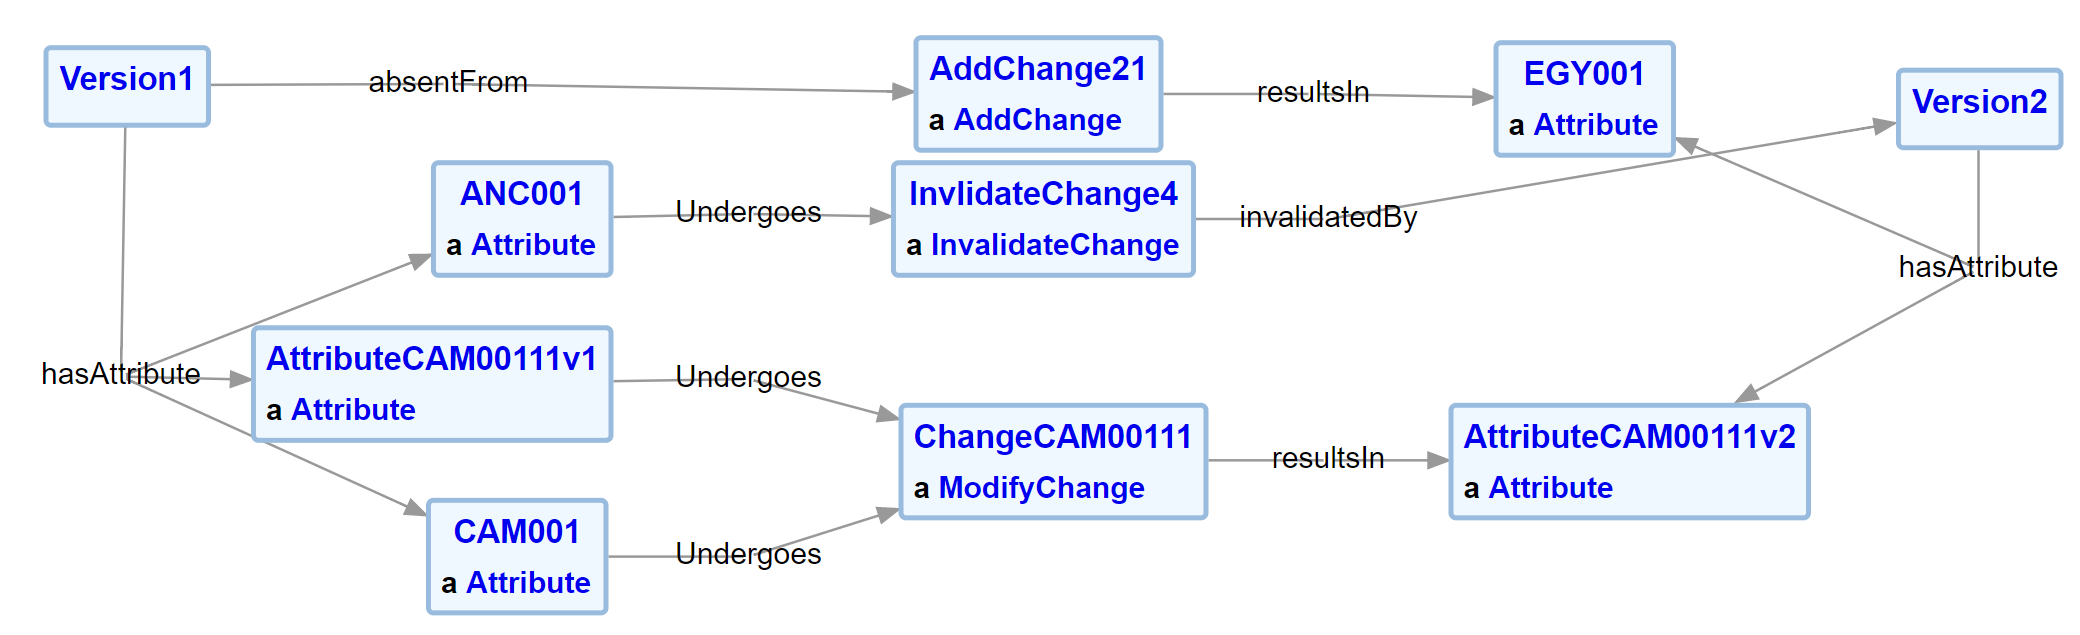
\includegraphics[scale=0.39]{figures/NobleVersion.png}
	\end{adjustbox}
\end{figure}
The \glspl{vergraph} presented in this section were created by extracting triples, using the code in Appendix \ref{extractor} from the associated \gls{log} which was covered in Chapter \ref{ch:changelog}.
The \mintinline{python}{extracting} function of the script extracts the JSON objects in every script tag, enters the values into an RDF graph, and then prints the graph out to a file.
The script has been generalized to process every JSON-LD encoded change log made in this thesis.
The statements making up the \gls{vergraph} could have alternately been published by writing out the triples directly instead of encoding them into a \gls{log}.
Figure \ref{NobleGraph1} displays a subgraph of the Noble Gas data set's \gls{vergraph} between Versions 1 and 2, highlighting each of the \gls{AIM} \glspl{change}.
Notice how the \gls{vergraph} differs from the provenance graph in Figure \ref{CAM001ProvGraph}.
The \gls{vergraph} unpacks the \textit{prov:wasRevisionOf} relationship into explicit components.
These components reveal more detailed differences between version 1 and 2 of CAM001 in the provenance graph which are the differing compilation activities.
\begin{figure}
	\centering
	\begin{adjustbox}{
		addcode=
			{\begin{minipage}{\width}}
			{
				\caption{Provenance graph for the CAM001 entry of the Noble Gas Database.  Other than the labels, the structure of each data object is very much the same.}
				\label{CAM001ProvGraph}
				\end{minipage}
			},
			rotate=90,
			center}
		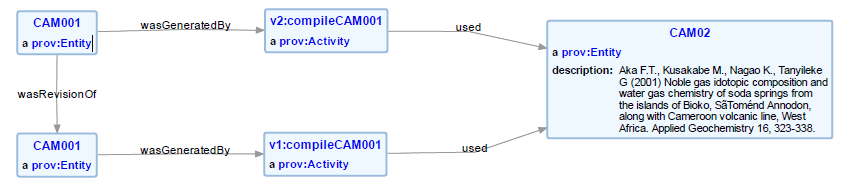
\includegraphics[scale=0.80]{figures/CAM001v1v2.png}
	\end{adjustbox}
\end{figure}
The \gls{log} encoded the triples in \gls{rdfa}, resulting in the \gls{attribute} ``AttributeCAM00111v2" to the right of the \gls{modify} change.
Because \gls{rdfa} does not naturally support multiple predicates while also conforming to the content structure of the \gls{log}, an \gls{attribute} was created to combine both the row and column identifier for the changing cell.
Separating the \glspl{attribute} would require multiple dedicated \gls{html} tags which don't appear along with content.
Including these tags would diverge from benefits of encoding triples as \glspl{attribute}.
Figure \ref{NobleGraph1} also shows that even though many columns are added when a new row is added, the row identifier can be used to summarize the columns additions.

Another modification to the implementation differs from the original versioning model.
The \gls{modify} construction defined in the model only covers the case where a single \gls{attribute} is sufficient to define a \gls{change}.
The \gls{modify} captured in spreadsheets describes a cell which requires a row and column identifier to indicate uniquely.
The implementation demonstrates that using multiple \glspl{attribute} is an allowable, sometimes necessary, construction.

Listing \ref{NGA} presents the statements in turtle format necessary to express that the entry EGY001 has been added to the data set from Version 1 to Version 2 as shown along the top of Figure \ref{NobleGraph1}.
The namespace for many of the \glspl{uri} is \textlangle http://rdfa.info/play/\textrangle.
\gls{rdfa} allows identifiers to refer to an element on the web page, and the web tool which generated the triples from \gls{rdfa}, therefore, used its \gls{url} as a namespace to produce a valid \gls{uri}.

\begin{listing}
	\begin{minted}[linenos, frame=lines, breaklines]{SPARQL}
<http://rdfa.info/play/Version1> a vo:Version ;
vo:absentFrom <http://rdfa.info/play/AddChange21> .
<http://rdfa.info/play/AddChange21> a <https://orion.tw.rpi.edu/~blee/VersionOntology.owl#AddChange> ;
vo:resultsIn <http://rdfa.info/play/Attribute21> .
<http://rdfa.info/play/Attribute21> a <https://orion.tw.rpi.edu/~blee/VersionOntology.owl#Attribute> ;
rdfs:label "EGY001"
<http://rdfa.info/play/Version2> a vo:Version ;
vo:hasAttribute <http://rdfa.info/play/Attribute21>
	\end{minted}
	\caption{Noble Gas Statements in Turtle for Addition 21 as an example for instantiating a versioning relation}
	\label{NGA}
\end{listing}

Figure \ref{CopperGraphVerGraph} shows a similar subgraph from the Copper data set \gls{vergraph}.
The \gls{vergraph} was assembled using an \gls{rdfa} \gls{log} and also displays a merged \gls{attribute} on the right side of the \gls{modify}.
In the full \gls{vergraph}, multiple of each \gls{change} is present, forming a zipper or ladder-like structure.
As a result, each \gls{add}, \gls{invalidate}, or \gls{modify} is given separate names for each instantiation.

\begin{figure}
	\centering
	\begin{adjustbox}{addcode={\begin{minipage}{\width}}{
					\caption{Versioning Graph representing the Copper Minerals linked data graph with selected entries of additions, invalidations, and modifications.}
					\label{CopperGraphVerGraph}					
					\end{minipage}},rotate=90,center}
		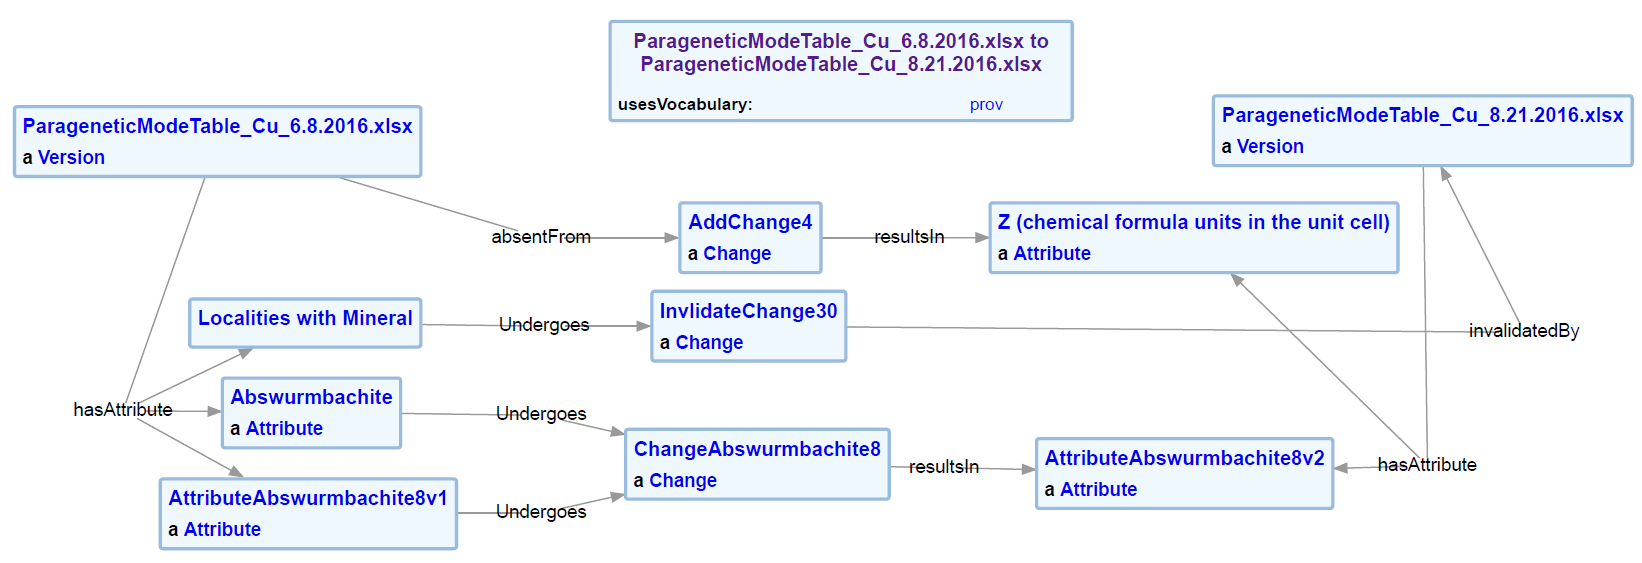
\includegraphics[scale=0.5]{figures/VersioningGraph2.png}%
	\end{adjustbox}
\end{figure}

\subsection{Graphs with Multiple Versions}\label{sec:multiver}

Figures \ref{NobleGraph1} and \ref{CopperGraphVerGraph} depict a comparison between only two \glspl{version}, but a project can contain more than two objects.
Case in point, Version 3 of the Noble Gas data set was released on July 11, 2017.
Figure \ref{NobleGraph2} shows a subgraph that contains changes from all three \glspl{version} of the Noble Gas data set.
\begin{figure}
	\centering
	\begin{adjustbox}{addcode={\begin{minipage}{\width}}{
					\caption{Versioning Graph representing the Noble Gas linked data graph with selected entries of additions, invalidations, and modifications after the publication of the third version.}
					\label{NobleGraph2}					
		\end{minipage}},rotate=90,center}
		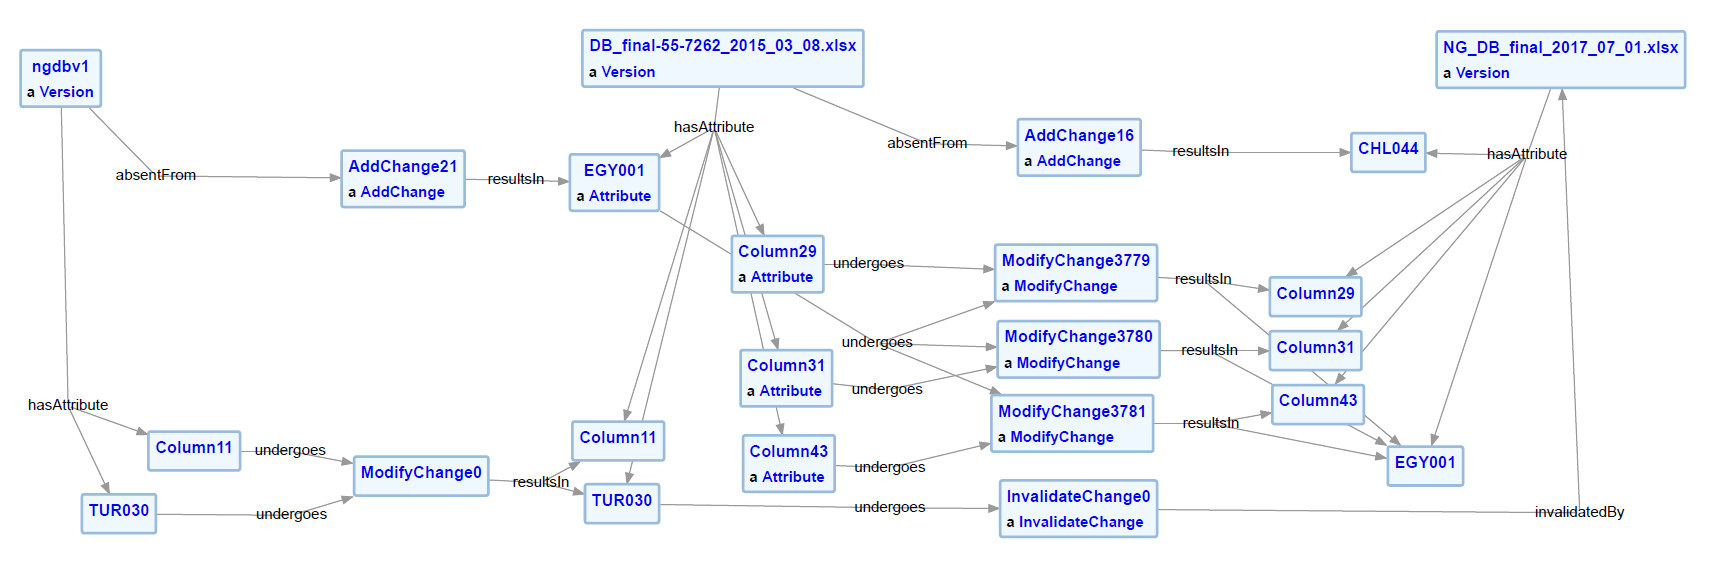
\includegraphics[scale=0.48]{figures/NobleVersion2.png}%
	\end{adjustbox}
\end{figure}
From Version 1 to Version 2 of the data, EGY001 becomes introduced as an \gls{attribute} into the data set.
This entry then undergoes a \gls{modify} in columns 29, 31, and 43 when comparing Version 2 and Version 3.
Entry TUR030 goes through a \gls{modify} change in column 11 from Version 1 to Version 2.
The entire row, however, becomes invalidated in Version 3.


Notice the difference in how Figure \ref{NobleGraph1} and Figure \ref{NobleGraph2} refer to columns.
Figure \ref{NobleGraph1} used \gls{linked} extracted from a \gls{log} employing \gls{rdfa}, forcing the row identifier and the column identifier into the same concept.
The way nesting works in \gls{rdfa} means that ChangeCAM00111 cannot back reference multiple concepts in a single statement, therefore AttributeCAM00111v2 was used to imply CAM001.
Figure \ref{NobleGraph2} used \gls{linked} extracted from a \gls{jsonld} encoded \gls{log}.
Since the \gls{log} can use explicit statements, the column identifier refers to the entire column and can be used to identify changes in the same column across multiple rows.

\section{Change Metric} \label{ch:distance}

Research Question 2 seeks to determine the extent of differences between two \glspl{version}.
Many versioning systems use dot-decimal identifiers to signify whether a change is large, medium, or small.
The exact requirements to determine change size differs widely across different domains and applications.
The \gls{vergraph} provides a new, more regular method to quantify change between objects using versioning operations.
The work done with \gls{gcmd} Keywords shows the qualitative relationship between version identifiers and change distance.
Work with the \gls{mbvl} data set then extends \gls{vo} to give more detailed accounting with the change capture method.

\subsection{Utilized Data Sets}

\subsubsection{Global Change Master Directory Keywords}

The \gls{gcmd} is a metadata repository used by \gls{nasa} to store records of its available data sets \cite{Miled:2001:GCM:372202.372324}.
They employ a set of keywords to make \gls{nasa} Earth Science data sets searchable.
These words tag and label datasets into strictly defined categories \cite{GCMDKey}.
\gls{gcmd} Keywords do not qualify as a standard web ontology since \gls{gcmd} Keywords do not constitute a class hierarchy.
The management team stored early versions of the keywords in Excel spreadsheets, later using a centralized distribution system, but data is not available prior to June 12, 2012.
The \gls{kms} now serves the keywords directly in a variety of formats.
Each version of the keywords, encoded in \gls{rdf}, was downloaded into separate files.
Only versions from June 12, 2012 and after were available, resulting in 9 version files.
Each keyword corresponds to a unique identifier, and when combined with a web namespace, resolves to a data description of the keyword.
Every identifier can be referred to per version by including the version's number at the web identifier's end, meaning that identifiers are consistent across versions.
The taxonomy uses the concepts \textit{skos:Broader} and \textit{skos:Narrower}, where skos refers to the \gls{skos} ontology name space, to form a tree hierarchy \cite{skos}.
The tree's root is the keyword, "Science Keywords."
The data set provides an interesting study case due its long sequence of versions and ready use of \gls{linked} technology \cite{Stevens2016}.

\subsubsection{Marine Biodiversity Virtual Laboratory Classifications} \label{sec:MBVL}

The \gls{mbvl}, based at Woods Hole Oceanographic Institution, provides data and services for the study of marine biology with an integrative approach \cite{mbvl}.
In the application studied, a choice of algorithm and taxonomy pairings must be tested on a known population in order to estimate their performance with an unknown microbial population.
The original sequences belong only to the species listed in Table \ref{species_table}.
The original population's census is not available to the author, and only the list of species is known, forming the first data set in this section.
These sequences are then grouped and classified by a specific taxonomy and algorithm pairing.
The workflow utilizes two taxonomies, the \gls{rdp} and the Silva taxonomy.
Using these databases, the \gls{spingo} or the \gls{gast} algorithms assign taxonomic ranks to each sequence.
The process produces four data sets, each using the same grouping identifiers and having the same size in each group.
Since the data sets have the same number of sequences, the primary differences between the data sets are the ranks assigned to each sequence.

\begin{table}
	\caption{List of species in the original population.}
	\label{species_table}
	\centering
	\setlength{\tabcolsep}{2pt}
	\begin{tabular}{|c|c|c|}
		\hline
		Acinetobacter baumannii & Actinomyces odontolyticus & Bacillus cereus \\
		Bacteroides vulgatus & Clostridium beijerinckii & Deinococcus radiodurans \\
		Enterococcus faecalis & Escherichia coli & Helicobacter pylori \\
		Lactobacillus gasseri & Listeria monocytogenes & Neisseria meningitidis\\
		Porphyromonas gingivalis & Propionibacterium acnes & Pseudomonas aeruginosa \\
		Rhodobacter sphaeroides & Staphylococcus aureus & Staphylococcus epidermidis\\
		Streptococcus agalactiae & Streptococcus mutans & Streptococcus pneumoniae \\
		\hline
	\end{tabular}
\end{table}

\section{Global Change Master Directory}

\subsection{Global Change Master Directory Versioning Graph}

The \gls{gcmd} establishes the context that each \textbf{manifestation} of their keyword list is related versions.
Since the unique identifier for each keyword remains the same across versions, the unique keyword identifier can be used to align a mapping across \glspl{version}.
\Glspl{add} and \glspl{invalidate} are detected by checking an identifier's presence within both versions.
Notice that the presence can be computed, as shown in lines 22 and 23 of \ref{app:gcmd}, without iterating through the data set.
A \gls{modify} occurs when a keyword's \textit{skos:Broader} property differs between adjacent \gls{version}.
The alignment assumes that there is not reason a keyword's preferred label would change, but still reports a value when it has new entries in the ``notes" property.
A difference indicates that the word has been moved to a different place within the taxonomy since identifiers do not change across versions and a keyword only has one parent concept.
\Glspl{change} over consecutive \glspl{version} can be collected into a single graph using the method in Section \ref{sec:multiver} to chain together \glspl{vergraph}.
A \gls{log} was generated for each pair of consecutive versions in \gls{gcmd} Keywords and embedded with \gls{jsonld}.
\Glspl{vergraph} for each adjacent \gls{version} was created by extracting \gls{jsonld} from the corresponding \gls{log}, and entering the triples into a Fuseki triple store.

\subsection{Connecting Change Counts to Identifiers} \label{gcmd_85}

The \gls{add}, \gls{invalidate}, and \gls{modify} counts for each transition are presented in Figure \ref{GCMDC1}.
Modify changes are labeled as Moves to differentiate between types of modifications when discussing Version 8.5.
The query used to extract the counts is found in Listing \ref{gcmd_list}.
Notice the sharp spike in \glspl{add} and \glspl{invalidate} when transitioning from Version 8.4.1 to 8.5.
The version identifiers indicate that at most a minor or technical change has occurred, but the counts of \gls{add} and \gls{invalidate} in this transition is more than triple the counts in either of the previous \textbf{major} transitions.
Not only should a small transition not produce changes of this quantity, but the data set's size is on the order magnitude of the recorded \glspl{invalidate}.
In addition, no \glspl{modify} are revealed, and even the root node "Science Keywords" has been invalidated.
Further investigation of the root word reveals that the name space for the keywords has changed from \mintinline{HTML}{http} to \mintinline{HTML}{https}.
To provide context, \gls{nasa} mandated a transition to secure protocols, and the group changed the name space to ensure the \glspl{uri} remained resolvable.
Since the identifiers are unique, the new name space means they no longer refer to the same object after the protocol change.
Because the keyword identifiers no longer match, the mapping approach results in the total invalidation of keywords from 8.4.1 and the addition of keywords from 8.5.
The dot decimal identifier for the transition from Version 8.4.1 to 8.5 does not match the number of changes in the \gls{vergraph}.

\begin{table}
	\caption{Global Change Master Directory Keyword Change Counts}
	\label{table:GCMD_main}
	\centering
	\begin{tabular}{|c|c|c|c|c|}
		\hline
		
		Transition&	Add&	Invalidate&	Modify&	Total\\\hline
		June 12, 2012 to 7.0&	310&	9&	22&	341\\
		7.0 to 8.0&	503&	6&	79&	588\\
		8.0 to 8.1&	277&	28&	22&	327\\
		8.1 to 8.2&	53&	1&	26&	80\\
		8.2 to 8.3&	58&	0&	13&	71\\
		8.3 to 8.4&	53&	0&	1&	54\\
		8.4 to 8.4.1&	86&	13&	8&	107\\
		\hline
	\end{tabular}
\end{table}
\begin{figure}[b]
	\centering
	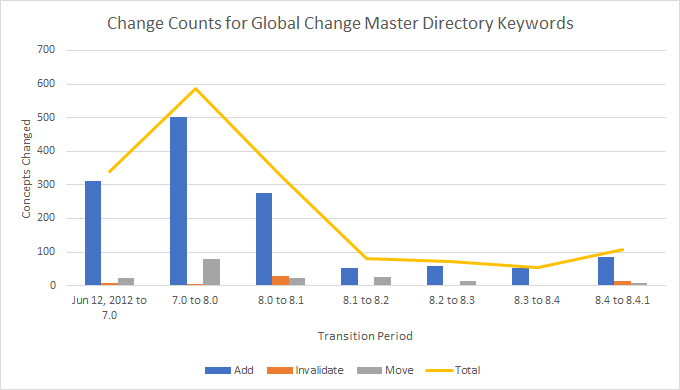
\includegraphics[scale=0.83]{figures/GCMDChartShort.png}
	\caption[Global Change Master Directory Keywords Change counts up to Version 8.4.1]{Add, Invalidate, and Modify counts from the beginning of the Keyword Management System to Version 8.4.1.}
	\label{GCMDC1}
\end{figure}

%\hfill \break

\begin{listing}
	\begin{minted}[linenos, frame=lines, breaklines]{sparql}
PREFIX vo:<http://orion.tw.rpi.edu/~blee/VersionOntology.owl>
PREFIX rdfs:<http://www.w3.org/2000/01/rdf-schema#>

SELECT ?p (COUNT (DISTINCT ?s) as ?count)
{
?s a ?p .
?p rdfs:subClassOf vo:Change .
} GROUP BY ?p
	\end{minted}
	\caption[Change count query.]{Query to compile the counts for each subclass of Change in a GCMD versioning graph.}
	\label{gcmd_list}
\end{listing}

Changing the mapping method to account for the new namespace provides a pathway to compare the perceived change by the producer as evidenced by the version identifier with the \gls{changedist} in the \gls{vergraph}.
To do this, the mapping treats identifiers with \mintinline{html}{http} and \mintinline{html}{https} the same as seen in lines 25 and 29 of Appendix \ref{app:gcmd85}.
The code breaks apart the \gls{uuid} from the \gls{uri} and uses the prior namespace or current namespace, respectively.
Differences in \gls{changedist} become much clearer after controlling for the altered name space in Figure \ref{GCMDC2}.
All revisions are dominated by \glspl{add}, but major version changes have counts around 300 to 500 while minor revisions are an order of magnitude smaller.
The transition from Version 8.4.1 to 8.5 also seems to follow this trend.
The \glspl{add} in ``8.4 to 8.4.1" in Figure \ref{GCMDC2} numbers almost a hundred, providing evidence that the trend of decreasing order of magnitudes may now continue as the granularity of the version identifier increases.

\begin{table}
	\caption{Difference in Version 8.5 mapping methods}
	\label{table:GCMD_8_5}
	\centering
	\begin{tabular}{|c|c|c|c|c|}
		\hline
		Mapping Method&	Add&	Invalidate&	Move&	Modify\\ \hline
		Standard&	3097&	3031&	0&	0\\
		Silent&	68&	2&	22&	0\\
		Bridged&	68&	2&	22&	3007\\		
		\hline
	\end{tabular}
\end{table}
\begin{figure}%[b]
	\centering
	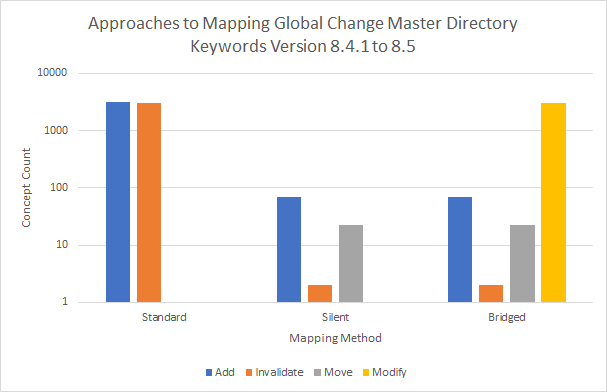
\includegraphics[scale=.9]{figures/GCMD8_5.png}
	\caption{Add, Invalidate, and Modify counts using different methods of mapping identifiers in Global Change Master Directory Keywords Version 8.4.1 to 8.5.}
	\label{GCMDC2}
\end{figure}


\section{Marine Biodiversity Virtual Laboratory}

\subsection{Variant Versioning Graph}

The experiment conducts activity over two phases in this procedure.
The first phase takes sequences from the original known population and feeds the sequences though a particular algorithm/taxonomy combination to produce a candidate classification.
Since the classifications for the known population sequences are unavailable, there is not sufficient context to perform a valid comparison with the candidate classifications.
The second phase compares the performances of each candidate classification of a algorithm/taxonomy pair.
The use of \gls{add}, \gls{invalidate}, and \gls{modify} varies slightly in this application since all the results use the same sequences.
A \gls{vergraph} utilizing just the sequence identifiers would only result in \textbf{modify} changes when taxonomic ranks differ since the sequence identifier exists in both data sets.
The mapping instead uses the sequence identifiers to align comparisons and then the taxonomic rank classification to determine the kind of \gls{change}.
If the right-hand result specifies more taxonomic ranks, the relationship is an \gls{add}, lines 200, 204, 216, and 226 in Appendix \ref{app:mbvl}.
If the left-hand result is more specific, then the relationship is classified as an \gls{invalidate}.
If both results have the same precision but the name differs, then the link is a \gls{modify}.
Otherwise, no \gls{change} is detected.
The \textbf{invalidations} and \textbf{modifications} were marked with `-{}-{}-' and `$>$$>$$>$' respectively in the function \mintinline{python}{get_output} of Appendix \ref{app:mbvl}.

Figure \ref{mbvl_chart} shows the changes detected when varying either the taxonomy or the classification algorithm.
\begin{figure}
	\centering
	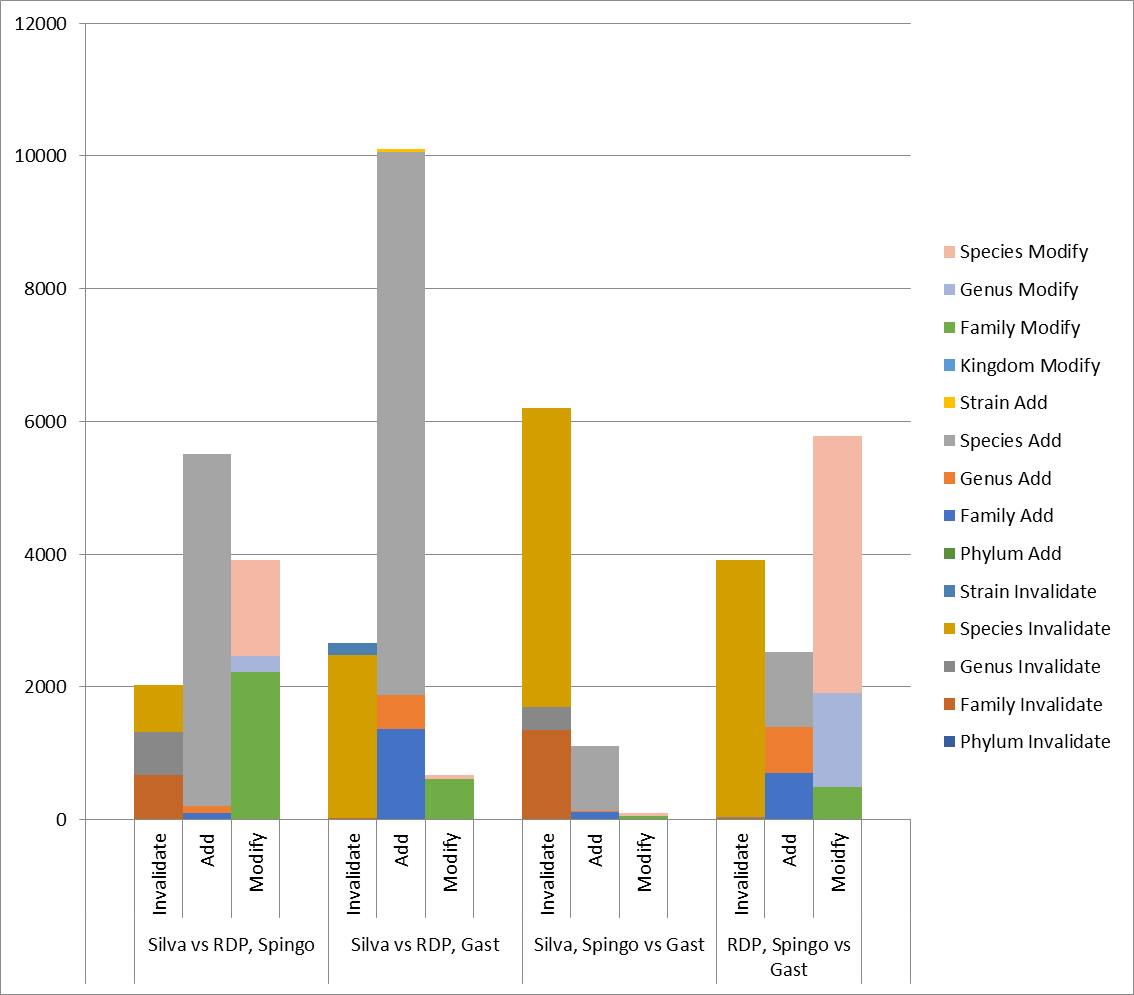
\includegraphics[scale=0.75]{figures/mbvl_chart.png}
	\caption{Compiled counts of \textbf{adds}, \textbf{invalidates}, and \textbf{modifies} grouped by taxonomic rank across algorithm and taxonomy combinations.}
	\label{mbvl_chart}
\end{figure}
Only the taxonomy or only the classifier differs in each comparison to control for overlapping influences that having both a different taxonomy and classifier may introduce.
Each bar indicates the total number of differences between sequences for a specific kind of \gls{change}.
The bars are further broken down by the taxonomic rank at which the difference occurred.
For example, in ``Silva vs RDP, Gast", a notable number of classifications differed at the species rank.
The graph also indicates that using the \gls{rdp} taxonomy often produces more precise classifications since both ``Silva vs RDP, Spingo" and ``Silva vs RDP, Gast" feature a larger number of \glspl{add} than any other change.
The classifier comparisons feature a high number of \glspl{invalidate}; however, ``RDP, Spingo vs Gast" also displays a higher number of \glspl{modify} than \glspl{invalidate}.

\section{Version Graph Discussion}

The \gls{vergraph} successfully addresses the concerns of Research Question 1 by capturing all the differences within the Noble Gas data set and within the Copper data set into a \gls{vergraph}.
Some additional concerns had to be addressed, such as dual \gls{attribute} identification, during the implementation of the versioning model.
The multiple files in the first version of the Noble Gas data set needed to be collected into a single concept in order to preserve the one-to-one relation between \glspl{version}.
The grouping simplifies the \gls{vergraph} structure as well as reduce the complexity of a \gls{log} encoding.

In Chapter \ref{ch:model}, there is only one \gls{attribute} on each side of the interaction.
Figure \ref{CopperGraphVerGraph}, however, shows two \glspl{attribute} used to characterize the \textit{vo:ModifyChange}.
While the model only shows one \gls{attribute}, it was found that in some applications, multiple \glspl{attribute} may be necessary to properly model a single \gls{change}.
The construction does not even need to have the same number \glspl{attribute} on both sides of the \gls{change}.
The flexibility becomes important when trying to model, for example, a single location entry being split into separate latitude and longitude entries.

The \gls{vergraph}'s construction allows multiple \glspl{version} to be linked together.
The \gls{vergraph} provides not only greater continuity than Schema.org's properties, but also greater detail than \gls{prov}'s versioning properties.
Continuity is important since many versioning \gls{linked} alternatives view version change as a single contained \textit{activity}.
When linking together multiple \glspl{version} using a \gls{vergraph}, the relationship between non-adjacent \glspl{version} becomes implied in the graph's structure.
The natural pathway between \glspl{attribute} in non-adjacent \glspl{version} holistically considers the relationships among all \glspl{attribute} along that path.
In comparison, other models only capture activity between the adjacent \glspl{version}.

The model struggles with discontinuous changes to an \gls{attribute} across multiple \glspl{version}.
Since the model does not capture when an \gls{attribute} doesn't change, it is possible for an \gls{attribute} in an earlier \gls{version} to become disconnected from later \glspl{version} due to inactivity.
For example, in Figure \ref{NobleGraph2}, column 31 of EGY001 becomes modified transitioning into the Version 3.
If that column underwent no activity in the next transition but changed from Version 4 to 5, the connection between all the column 31s would no longer be continuous.
This poses a problem for executing queries in a triple store which rely on graph traversals, but no path exists between disconnected \glspl{attribute}.

\subsection{Version Identification}

The versioning process discovered a discrepancy in the identifier assignment in the \gls{gcmd} Keywords taxonomy.
The original analysis was intended to determine if dot-decimal identifiers would reflect an order of magnitude division among the change counts of the \gls{vergraph}.
According to the \textit{Keyword Governance and Community Guide Document} \cite{gcmd_gov}, ``Full GCMD keywords list releases get a new major version number (e.g., 8.0). Incremental releases for updates to topics, terms, and variables get a new minor version number (e.g., 8.1).”
The change counts for Versions `June 12, 2012' to 8.4.1 demonstrates a threshold of \glspl{change} necessitating a full keywords list release.
The document does not explain the purpose or distinguishing qualities of \glspl{version} with a new revision number, 8.4.1.
Version 8.5, however, was named with respect to perceived taxonomy changes and did not consider underlying \gls{linked} practice revisions.
The conclusion can be obtained by looking at \ref{GCMDC2} and noticing that the only matching approach without a bar equal to the size of the entire data set is the `Silent' approach.
For a purely \gls{uri} based comparison in `Standard', Version 8.5 definitely falls under the category of full release since an entirely new list of words is released.
Users using the `Bridged' approach would also see a new full release because all old words have had the \glspl{uri} edited.
Version name assignment based on producer perception and not allowing users to assess change measures is concerning.
Making sure that data consumers have the ability to assess change in data sets when the requirements for change differs between producer and consumer must be addressed.

The analysis does not to claim that \gls{changedist} should be the sole mechanism in determining version identifiers.
The counts, however, can provide a more quantitative method to compare version differences.
In Figure \ref{GCMDC1}, the yellow line indicates the total changes made to the data set, performing a similar function as the major/minor/revision version identifier.
Breaking up the changes into types reveals additions dominate manipulations to the data set.
\Gls{add}, \gls{invalidate}, and \gls{modify} provides deeper insight into how a data set is changing, but some \glspl{change} can be more impactful than others which this model does not capture.

\subsection{MBVL Analysis}

In Section \ref{ch:distance}, the versioning process was used to compare the performance of different taxonomy and algorithm combinations.
The data set diverges from many of the common understandings of \glspl{version} since each of the \glspl{version} are not sequential and are largely independent.
The data set of species names in the initial population would not have produced very meaningful results if applied to the versioning model since it lacked sufficient data to map the other data sets together well.

In Figure \ref{mbvl_chart}, the first set of columns in the Silva taxonomy results are versioned against \gls{rdp} using the \gls{spingo} algorithm.
The naming reflects the orientation in the \gls{vergraph} so Silva forms the left-hand version and \gls{rdp} would be the right-hand \gls{version}.
In this comparison, using the \gls{rdp} taxonomy seems to provide more accurate results, most specifically at the species level.
The taxonomies also disagree fairly often at the species and family ranks.
Switching to the \gls{gast} algorithm in the second set of columns, \gls{rdp} once again demonstrates a noticeably greater accuracy in species classification.
There are also significantly fewer disagreements using the \gls{gast} algorithm between the two taxonomies.
Looking at the third set of columns, Silva demonstrates greater accuracy classifications under the \gls{spingo} algorithm than under \gls{gast}.
Over four thousand of these entries can be classified to the species level when \gls{gast} cannot.
In the fourth set of columns, \gls{rdp} appears to perform better with \gls{spingo} than \gls{gast}.
However, the comparison is dominated by a much larger number of disagreements between almost six thousand entries, primarily at the species rank.
On closer inspection, this disagreement is explained by \gls{gast} classifying the species for a number of entries as ``uncultured bacterium".
This analysis presents evidence that using the \gls{rdp} taxonomy with the \gls{spingo} algorithm will produce the most accurate classification results.

\section{Summary}

The results in this chapter implements the versioning model and demonstrates the process and challenges experienced in this endeavor.
The entries in a data set is separated into groups of \glspl{add}, \glspl{invalidate}, \glspl{modify}, and unmodified by their \glspl{attribute}.
These operational groups organizes the data into a form to publish into a \gls{vergraph}.
The approach used to create the \gls{vergraph} involves extracting the \gls{linked} from a marked up \gls{log}.
The decision resulted in constrained representations of the \gls{vergraph}, resulting from demands of the encoding methods.
\Glspl{vergraph} created using freer form statements, such as the one in Figure \ref{NobleGraph2}, demonstrate an opportunity enable querying over different dimensions of the data.
Changes for specific columns can be queries as easily as individual rows.

The ability to link \glspl{change} of multiple \glspl{version} together results as a side effect of the model construction.
Continuously linked \glspl{change} opens up avenues of exploration to follow change as it propagates through \glspl{version}.
While \glspl{log} will provide a more focused comparison, a triple store with a multi-version graph would give a view of the work through time.
Considering the Noble Gas data set's \gls{vergraph}'s size, many \glspl{version} may be difficult to store with large, volatile data sets.

The \gls{mbvl} data set demonstrates a case where \glspl{vergraph} can be used to compare the performance of different taxonomy/algorithm pairings.
The ability derives from sub-classing each of the \gls{AIM} \glspl{change} to give a better perspective where the pairings differed.
This approach of extending the \glspl{vergraph} adds domain knowledge to the version comparison and helps contextualize the observed differences.
